\section{АНАЛИЗ ПРЕДМЕТНОЙ ОБЛАСТИ}
\label{sec:analysis}

При проектировании программного продукта, который решает реальные задачи пользователя, очень важно выяснить главный фукционал и свойства продукта, чтобы сервис отвечал запросам пользователей и производство продукта было оправдано.

Требования к ПО определяют, какие свойства и характеристики оно должно иметь для удовлетворения потребностей пользователей и других заинтересованных лиц. Однако сформулировать требования к сложной системе не так легко. В большинстве случаев будущие пользователи могут перечислить набор свойств, который они хотели бы видеть, но никто не даст гарантий, что это — исчерпывающий список. Кроме того, часто сама формулировка этих свойств будет непонятна большинству программистов.

Чтобы ПО было действительно полезным, важно, чтобы оно удовлетворяло реальные потребности людей и организаций, которые часто отличаются от непосредственно выражаемых пользователями желаний. Для выявления этих потребностей, а также для выяснения смысла высказанных требований приходится проводить достаточно большую дополнительную работу, которая называется анализом предметной области или бизнес-моделированием, если речь идет о потребностях коммерческой организации. В результате этой деятельности разработчики должны научиться понимать язык, на котором говорят пользователи и заказчики, выявить цели их деятельности, определить набор задач, решаемых ими. В дополнение стоит выяснить, какие вообще задачи нужно уметь решать для достижения этих целей, выяснить свойства результатов, которые хотелось бы получить, а также определить набор сущностей, с которыми приходится иметь дело при решении этих задач. Кроме того, анализ предметной области позволяет выявить места возможных улучшений и оценить последствия принимаемых решений о реализации тех или иных функций.

После этого можно определять область ответственности будущей программной системы — какие именно из выявленных задач будут ею решаться, при решении каких задач она может оказать существенную помощь и чем именно. Определив эти задачи в рамках общей системы задач и деятельностей пользователей, можно уже более точно сформулировать требования к ПО.

Анализом предметной области занимаются системные аналитики или бизнес-аналитики, которые передают полученные ими знания другим членам проектной команды, сформулировав их на более понятном разработчикам языке. Для передачи этих знаний обычно служит некоторый набор моделей, в виде графических схем и текстовых документов.

Анализ деятельности крупной организации, такой как банк с сетью региональных отделений, нефтеперерабатывающий завод или компания, производящая автомобили, дает огромные объемы информации. Из этой информации надо уметь отбирать существенную, а также уметь находить в ней пробелы — области деятельности, информации по которым недостаточно для четкого представления о решаемых задачах. Значит, всю получаемую информацию надо каким-то образом систематизировать.

\subsection{Системы электронного документооборота}
\label{sec:analysis:serv_arch}

Официального определения системы электронного документооборота (СЭД), утвержденного стандартом, не существует. По сути, СЭД – это система, позволяющая автоматизировать основные процедуры делопроизводства компании. Она охватывает процессы создания, обработки, тиражирования, передачи, хранения документов, контроля над их исполнением и предназначена для эффективного управления предприятием.


\begin{figure}[h!]
	\centering
	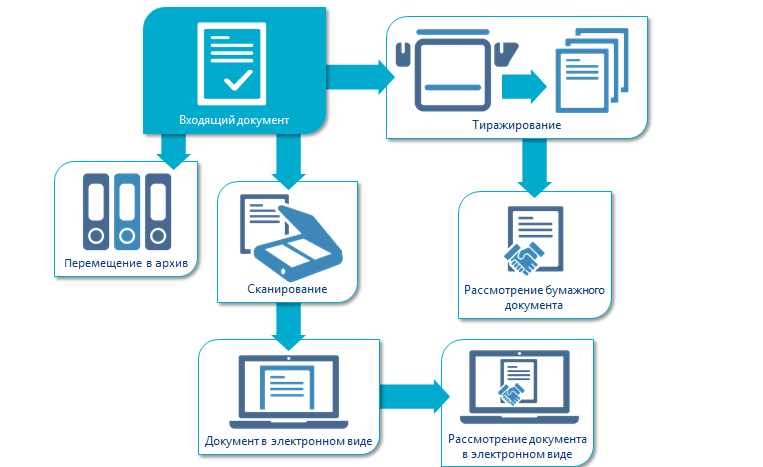
\includegraphics[scale=0.78]{sed_in_russia_today.png}
	\caption{Схема использования СЭД}
\end{figure}

При внедрении СЭД на предприятии обычно ставят следующие цели:
\begin{itemize}
	\item сокращение или полный отказ от бумажного документооборота; 
	\item создание единой информационной базы компании; 
	\item снижение риска утери документа; 
	\item структурирование всей документации по утвержденной номенклатуре;
	\item повышение дисциплины среди сотрудников благодаря возможности отслеживания деятельности исполнителя конкретного документа;
	\item контроль над исполнением документов в соответствии с резолюциями руководителя;
	\item повышение эффективности работы компании.
\end{itemize}

СЭД – один из главных информационных ресурсов компании, который используется для работы с самыми разными видами и типами документов, интегрируется с другими деловыми системами. Традиционный для СЭД функционал, по мнению экспертов компании «1С», расширяется в направлении автоматизации совместной работы сотрудников.

Как и любой инструмент, СЭД нужно применять по назначению и тогда, когда это действительно необходимо компании. Только в этом случае внедрение системы будет эффективно и принесет реальную пользу.

Определить эффективность внедрения СЭД в цифровом выражении достаточно сложно. Компанией DIRECTUM на основе собственной методики были выделены ключевые эффекты от внедрения СЭД на предприятии \cite{directum}. При этом величина эффекта зависит от того, является ли компания крупным предприятием с несколькими филиалами или небольшим предприятием, расположенном в одном офисе. Потенциальные выгоды следующие:

\begin{itemize}
  \item[1] \textbf{Снижение материальных затрат:}
	
	\begin{itemize}
	  \item небольшое предприятие – на 5\%;
	  \item крупное предприятие с несколькими филиалами – на 20\%.
	\end{itemize}

  \item[2] \textbf{Экономия на базовых процессах} – исходящие и входящие документы, организационно-распорядительный документооборот, контроль исполнения поручений:
	
	\begin{itemize}
	  \item небольшая компания – от 8 до 15\%;
	  \item крупное предприятие – до 50\%.
	\end{itemize}
	
  \item[3] \textbf{Экономия на конкретных операциях}, не привязанных к процессам, – поиск документов, обеспечение доступа к ним и т.д. – от 3 до 24\% в зависимости от стиля работы с документами и от организации системы их хранения. Если создать общедоступное хранилище электронных документов с четко прописанными регламентами работы и хранения, правами доступа к ним, то эффект для компании будет максимальным.

  \item[4] \textbf{Снижение рисков.} Этот эффект касается стратегических показателей и меньше всего поддается формальному расчету. В некоторых случаях СЭД позволяет снизить риски просрочки согласования и заключения договоров до 60\%.

\end{itemize}

По оценкам экспертов, внедрение СЭД на предприятии окупается в среднем за срок от 3 месяцев до 3 лет \cite{ecm_journal}.


\subsection{Анализ рынка СЭД}
\label{sec:analysis:sed_market}

По оценке TAdviser, в 2016 году положительная динамика российского рынка СЭД сохранилась. Как и годом ранее она составила 10\%, при этом объем рынка в рублевом выражении увеличился до 41,6 млрд рублей \cite{tadviser_market1}.

На продолжающийся рост рынка влияет как общее восстановление экономики, так и отдельные драйверы. Для сферы СЭД/ECM – это набирающий обороты процесс импортозамещения, курс на цифровую экономику, повышение мобильности и стремительное развитие новых технологий.

\begin{figure}[h!]
\centering
	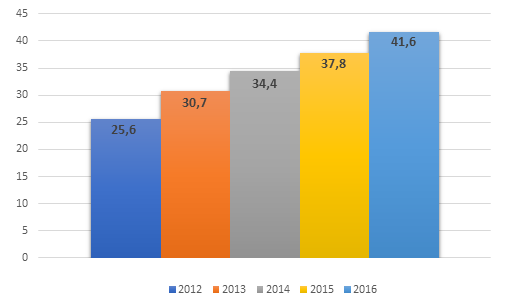
\includegraphics[scale=1.2]{Market_sed.png}
	\caption{Динамика российского рынка СЭД, млрд руб.}
\end{figure}
\clearpage
